%\documentclass[first=dgreen,second=purple,logo=yellowexc]{aaltoslides}
%\documentclass{aaltoslides} % DEFAULT
%\documentclass[first=purple,second=lgreen,logo=redque,normaltitle,nofoot]{aaltoslides} % SOME OPTION EXAMPLES
\documentclass[normaltitle,first=orange,second=red,leqno]{aaltoslides}

\usepackage{natbib}
\bibliographystyle{plainnat}
\setcitestyle{numbers,open={[},close={]},comma}
\usepackage{physics}
% \usepackage[finnish]{babel}
\usepackage[english]{babel}

\usepackage[latin9]{inputenc}
\usepackage[T1]{fontenc}
\usepackage{graphicx}
\usepackage{amssymb,amsmath}
\usepackage{url}
\usepackage{lastpage}
\usefonttheme{professionalfonts}
\usepackage{tikz}
\usepackage{hyperref}
\usepackage{algorithm}
\usepackage{algpseudocode}
\usepackage{chessboard}
\usepackage{caption}

\usetikzlibrary{patterns,arrows,decorations.pathreplacing}

\DeclareMathOperator*{\osc}{osc}
\DeclareMathOperator*{\essliminf}{ess\,liminf}
\DeclareMathOperator*{\esssup}{ess\,sup}
\DeclareMathOperator*{\essinf}{ess\,inf}
\DeclareMathOperator*{\eliminf}{ess\,lim\,inf}
\DeclareMathOperator*{\elimsup}{ess\,lim\,sup}
\DeclareMathOperator*{\diam}{diam}
\DeclareMathOperator*{\spt}{spt}
\DeclareMathOperator*{\dist}{dist} \DeclareMathOperator*{\dive}{div}
\DeclareMathOperator*{\Lip}{Lip}
\DeclareMathOperator*{\lip}{lip}
\DeclareMathOperator{\Mod}{Mod}
\DeclareMathOperator{\Capc}{Cap}
\DeclareMathOperator{\rcapa}{cap}
\DeclareMathOperator*{\supp}{supp}

\def\vint_#1{\mathchoice%
          {\mathop{\kern 0.2em\vrule width 0.6em height 0.69678ex depth -0.58065ex
                  \kern -0.8em \intop}\nolimits_{\kern -0.4em#1}}%
          {\mathop{\kern 0.1em\vrule width 0.5em height 0.69678ex depth -0.60387ex
                  \kern -0.6em \intop}\nolimits_{#1}}%
          {\mathop{\kern 0.1em\vrule width 0.5em height 0.69678ex depth -0.60387ex
                  \kern -0.6em \intop}\nolimits_{#1}}%
          {\mathop{\kern 0.1em\vrule width 0.5em height 0.69678ex depth -0.60387ex
                  \kern -0.6em \intop}\nolimits_{#1}}}

\newcommand{\art}[6]{{\sc #1, \rm #2, \it #3 \bf #4 \rm (#5), \mbox{#6}.}}
\newcommand{\book}[3]{{\sc #1, \it #2, \rm #3.}}
\newcommand{\AND}{{\rm and }}
\newcommand{\p}{{$p\mspace{1mu}$}}
\newcommand{\q}{{$q\mspace{1mu}$}}
\newcommand{\Np}{N^{1,p}}
\newcommand{\Nploc}{N^{1,p}\loc}
\newcommand{\Wp}{W^{1,p}}
\newcommand{\Wploc}{W^{1,p}\loc}
\newcommand{\Nq}{N^{1,q}}
\newcommand{\Nqloc}{N^{1,q}\loc}
\newcommand{\Wq}{W^{1,q}}
\newcommand{\Wqloc}{W^{1,q}\loc}
% \newcommand{\grad}{\nabla}
\newcommand{\Om}{\Omega}
\newcommand{\loc}{\mathrm{loc}}
\newcommand{\Lipc}{{\Lip_c}}
\newcommand{\eps}{\varepsilon}
\newcommand{\pip}{\varphi}
\newcommand{\BV}{\mathrm{BV}}
\newcommand{\liploc}{\mathrm{Lip}_{\mathrm{loc}}}
\newcommand{\ch}{\text{\raise 1.3pt \hbox{$\chi$}\kern-0.2pt}}
\newcommand{\ave}[1]{\langle #1\rangle}
%\AtBeginSection[]
%{
%  \begin{frame}
%    \frametitle{Table of Contents}
%    \tableofcontents[currentsection]
%  \end{frame}
%}
\newcommand{\thesiscolor}{orange}


\title{Teaching masked diffusion language models to generate chess puzzles with reinforcement learning}




\author[Lyhyt nimi]{Aatu Selkee}
% \institute[MSA]{Matematiikan ja systeemianalytiikan laitos\\Aalto-yliopisto}

\aaltofootertext{Aatu Selkee}{July 3, 2026}{\insertframenumber{} / \inserttotalframenumber}%{\arabic{page}/\pageref{LastPage}\ }

\date{\small{July 3, 2026} \\ Advisor Adjunct Prof. Eric Malmi\\Supervisor Prof. Nuutti Hyv\"onen}

\setbeamercovered{transparent}
\setcounter{tocdepth}{1}







% Define custom colors for visualization
\definecolor{maskgray}{RGB}{220,220,220}
\definecolor{newred}{RGB}{255,200,200}
\definecolor{oldblue}{RGB}{200,220,255}
\definecolor{diffgreen}{RGB}{200,255,200}

% Define helper commands for highlighted boxes
\newcommand{\mask}{\texttt{[MASK]}}
\newcommand{\graybox}[1]{\colorbox{maskgray}{#1}}
\newcommand{\redbox}[1]{\colorbox{newred}{#1}}
\newcommand{\bluebox}[1]{\colorbox{oldblue}{#1}}
\newcommand{\greenbox}[1]{\colorbox{diffgreen}{#1}}







\begin{document}


\aaltotitleframe

\begin{frame}{Table of Contents}
    \tableofcontents
\end{frame}


\section{Introduction}

\begin{frame}
\begin{center}
\Huge{\color{\thesiscolor} Introduction}
\end{center}
\end{frame}

\begin{frame}{Introduction}
    \begin{itemize}
        % \item<1-> Traditionally, creativity has been thought of as a key component of machine intelligence \cite{colton2012computationalcreativity}.
        \item<1-> In this thesis, we train a model to generate chess puzzles with certain properties.
        \item<2-> Chess puzzle generation requires creativity and reasoning.
        \item<3-> Contributions:
        \begin{itemize}
            \item Demonstrate the effectiveness of masked diffusion models.
            \item Demonstrate that chess puzzle generation can be conditioned on specific themes.
            \item Demonstrate that masked diffusion models can be improved via reinforcement learning.
            \item Demonstrate that auxiliary task of best move prediction improves puzzle generation.
        \end{itemize}
        \item<4-> We follow the work of \citeauthor{feng2025generatingcreativechesspuzzles}.
    \end{itemize}
\end{frame}


\section{Background}

\begin{frame}
\begin{center}
\Huge{\color{\thesiscolor} Language modelling}
\end{center}
\end{frame}

\begin{frame}{Language modelling}
    \begin{itemize}
        \item<1-> In language modelling, autoregressive language models are the most common paradigm currently.
        \item<2-> In recent years, diffusion models, have become very popular for continuous problems, such as image, video or audio generation.
        \item<3-> Discrete diffusion, in particular masked diffusion, has become a compelling alternative for large language models (LLMs).
    \end{itemize}
\end{frame}


\begin{frame}{Autoregressive LLM vs. Masked Diffusion}
    \begin{columns}[T]
        
        % ==========================================
        % LEFT COLUMN: Autoregressive Model
        % ==========================================
        \begin{column}{0.43\textwidth}
            \centering
            \textbf{\large Autoregressive LLM}\\[0.1cm]
            
            \raggedright
            \footnotesize
            \textbf{Step 1:}
            \redbox{Machines}\\[0.25cm]
            
            \textbf{Step 2:}
            \bluebox{Machines} \redbox{take}\\[0.25cm]
            
            \textbf{Step 3:}
            \bluebox{Machines take} \redbox{me}\\[0.25cm]
            
            \textbf{Step 4:}
            \bluebox{Machines take me} \redbox{by}\\[0.25cm]

            \textbf{Step 5:}
            \bluebox{Machines take me by} \redbox{surprise}\\[0.25cm]
            
            \textbf{\dots}\\[0.25cm]
            
            \textbf{Step 8:}
            \bluebox{Machines take me by}\\
            \bluebox{surprise with great} \redbox{frequency.}\\[0.4cm]

            -- \textit{Alan Turing}
        \end{column}

        % ==========================================
        % RIGHT COLUMN: Masked Diffusion Model
        % ==========================================
        \begin{column}{0.57\textwidth}
            \centering
            \textbf{\large Masked Diffusion}\\
            
            \begin{columns}[T]
                % Arrows Column
                \begin{column}{0.05\textwidth}
                    \centering
                    \vspace{1.2cm}
                    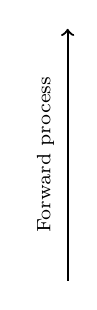
\begin{tikzpicture}
                        % Forward Process Arrow (Bottom to Top)
                        \draw[<-, thick, black] (0, 3.2) -- (0, 0) 
                            node[midway, xshift=-8pt, rotate=90] {\scriptsize Forward process};
                    \end{tikzpicture}
                \end{column}
                
                % Text Column
                \begin{column}{0.8\textwidth}
                    \raggedright
                    \footnotesize
                    \textbf{Step 1:} \graybox{\mask} \graybox{\mask} \graybox{\mask} \graybox{\mask} \graybox{\mask} \graybox{\mask} \graybox{\mask} \graybox{\mask}\\[0.25cm]
                    
                    \textbf{Step 2:} \greenbox{Machines} \graybox{\mask} \greenbox{me} \graybox{\mask} \graybox{\mask} \graybox{\mask} \greenbox{great} \graybox{\mask}\\[0.25cm]
                    
                    \textbf{Step 3:} \greenbox{Machines} \graybox{\mask} \greenbox{me by surprise} \graybox{\mask} \greenbox{great} \graybox{\mask}\\[0.25cm]
                    
                    \textbf{Step 4:} \greenbox{Machines take me by surprise}\\
                    \greenbox{with great frequency.}
                \end{column}

                
                \begin{column}{0.15\textwidth}
                    \centering
                    \vspace{1.2cm}
                    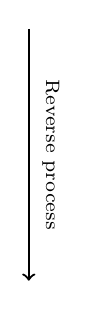
\begin{tikzpicture}
                        % Reverse Process Arrow (Top to Bottom)
                        \draw[->, thick, black] (0.4, 3.2) -- (0.4, 0) 
                            node[midway, xshift=8pt, rotate=270] {\scriptsize Reverse process};
                    \end{tikzpicture}
                \end{column}
            \end{columns}
        \end{column}
        
    \end{columns}
\end{frame}

\begin{frame}{Autoregressive LLM vs. Masked Diffusion}
    \begin{table}
        \centering
        \caption{Comparison of Autoregressive LLMs and Masked Diffusion Models.}
        \begin{tabular}{|p{0.22\textwidth}|p{0.3\textwidth}|p{0.35\textwidth}|}
            \hline
             & \textbf{Autoregressive LLMs} & \textbf{Masked Diffusion Models} \\
            \hline\hline
            \textbf{Generation Method} & Left-to-right & Random order \\
            \hline
            \textbf{Inference Speed} & Linear in output length (Slow) & Manual control over denoising steps (Fast) \\
            \hline
            \textbf{Training Speed} & Slow & Even slower (16x more pretraining \cite{nie2025scalingmaskeddiffusionmodels}) \\
            \hline
            \textbf{Performance} & Great & Similar \\
            \hline
        \end{tabular}
    \end{table}
\end{frame}

\begin{frame}
\begin{center}
\Huge{\color{\thesiscolor} Masked Diffusion}
\end{center}
\end{frame}

\begin{frame}{Masked diffusion}
    \begin{itemize}
        \item<1-> We follow the formalization of \citeauthor{shi2025simplifiedgeneralizedmaskeddiffusion}.
        % \item<2-> To train a masked diffusion model, a forward process is needed, where tokens are iteratively converted into mask tokens \mask.
        % \item<3-> Time interval $[0, 1]$ is divided into $T$ steps.
        % \item<2-> To begin with, we consider just one token $y$, which is one-hot encoded.
        % \item<3-> The forward process of the whole sequence is determined using the conditional independence of token transitions on each step.
        \item<2-> Forward process turns sequences of real tokens into mask tokens.
        \item<3-> Generation of new sequences requires a reverse process.
    \end{itemize}
\end{frame}

% \begin{frame}{Discrete-time forward process}
%     \begin{itemize}
%         \item<1-> For time $t(i)$, the transition from $y_{t(i - 1)}$ to $y_{t(i)}$ is determined by the following transition matrix:
%         \begin{equation}
%             Q_i = (1 - \beta_i) I + \beta_i\bold{1}e_m^\top\in\mathbb{R}^{(m + 1)\cross(m + 1)},
%         \end{equation}
%         where $\bold{1}\in\mathbb{R}^{m + 1}$ is the vector of ones, $e_m$ is the basis vector of the mask token and $\beta_i$ determines the probability that $y_{t(i - 1)}$ is transformed into the masked state.
%         \item<2-> The state $y_{t(i)}$ distribution from an uncorrupted one-hot encoded state $y$ is:
%         \begin{equation*}
%             q(y_{t(i)} | y) = \text{Cat}(y_{t(i)}; \bar{Q}_i^\top y), \quad\bar{Q}_i = \alpha_i I + (1 - \alpha_i)\bold{1}e_m^\top,
%         \end{equation*}
%         where $\alpha_i = \prod_{j=1}^{i}(1 - \beta_j)$.
%     \end{itemize}
% \end{frame}

% \begin{frame}{Continuous-time forward process}
%     \begin{itemize}
%         \item<1-> We generalize to continuous-time by taking the limit $T\rightarrow\infty$:
%         \begin{equation*}
%             \bar{Q}(t) = \alpha_tI + (1 - \alpha_t)\bold{1}e_m^\top, \quad\text{where }\alpha_t = \exp\left( -\int_{0}^{t}\beta(s)\mathrm{d}s \right).
%         \end{equation*}
%         \item<2-> The masking schedule $\alpha_t$ defines the process. We use the linear schedule:
%         \begin{equation*}
%             \alpha_t = 1 - t.
%         \end{equation*}
%         \item<3-> Many other masking schedules exist, but for every masking schedule, we have $\alpha_0 = 1$, $\alpha_1 = 0$ and $\alpha_t\in[0, 1]$.
%         \item<4-> We then get the distribution of $y_t$ conditioned on $y_s, s < t$:
%         \begin{equation*}
%             q(y_t | y_s) = \text{Cat}(y_t; \bar{Q}(s, t)^\top y_s), \quad\bar{Q}(s, t) = \frac{\alpha_t}{\alpha_s}I + \left(1 - \frac{\alpha_t}{\alpha_s}\right)\bold{1}e_m^\top.
%         \end{equation*}
%     \end{itemize}
% \end{frame}

\begin{frame}{Forward process}
    \begin{itemize}
        \item<1-> An uncorrupted token sequence is converted into a sequence of mask tokens \mask in $T$ steps.
        \item<2-> The amount of tokens converted to mask tokens is determined by a masking schedule $\alpha_t$.
        \begin{itemize}
            \item We use a linear schedule, where approximately equal number of tokens are masked on every step.
            \item Many other masking schedules exist, but all must begin from an uncorrupted token sequence and end at a masked sequence.
        \end{itemize}
    \end{itemize}
\end{frame}

% \begin{frame}{Reverse process}
%     \begin{itemize}
%         \item<1-> During the reverse process, we reverse the masking process and attempt to convert each masked token into the true token.
%         \item<2-> One can derive the following expression for the reverse process:
%         \begin{align*}
%             q(y_s | y_t, y) &= \text{Cat}(y_s; \bar{R}^{y}(t, s)^\top y_t), \\
%             \bar{R}^{y}(t, s) &= I + \frac{\alpha_s - \alpha_t}{1 - \alpha_t}e_m(y - e_m)^\top \text{ and } s < t.
%         \end{align*}
%         \item<3-> Hence, if we know the original token sequence $y$ that has no masking, we can compute the distribution of a step closer to the unmasked state.
%         \item<4-> However, $y$ is unknown when sampling new sequences.
%     \end{itemize}
% \end{frame}

% \begin{frame}{Reverse process}
%     \begin{itemize}
%         \item<1-> To solve this problem, we introduce the denoising network $\mu_\theta(y_t, x)$, which given a noisy state $y_t$ and a prompt $x$, outputs a probability distribution over the vocabulary for each masked token.
%         \item<2-> Using this network, we define the distribution for $y_s$ as:
%         \begin{equation*}
%             p_\theta(y_s | y_t, x) = q(y_s | y_t, \mu_\theta(y_t, x)) = \text{Cat}(y_s; \bar{R}^{\mu_\theta(y_t, x)}(t, s)^\top y_t).
%         \end{equation*}
%         \item<3-> Intuitively, if $y_t$ is a mask token, we sample a new token from $\mu_\theta(y_t, x)$ with probability $p_{\text{unmask}}^{(s)} = \frac{\alpha_s - \alpha_t}{1 - \alpha_t}$, otherwise we keep the mask token. Unmasked tokens remain the same.
%     \end{itemize}
% \end{frame}

\begin{frame}{Reverse process}
    \begin{itemize}
        \item<1-> Masked token sequences are converted into real tokens.
        \item<2-> Using Bayes rule on the forward process, a distribution over tokens can be obtained.
        \item<3-> Using a denoising network $\mu_\theta(y_t, x)$, we have the following distribution:
        \begin{align*}
            p_\theta(y_s | y_t, x) &= \text{Cat}(y_s; \bar{R}^{\mu_\theta(y_t, x)}(t, s)^\top y_t) \\
            \bar{R}^{\mu_\theta(y_t, x)}(t, s) &= I + \frac{\alpha_s - \alpha_t}{1 - \alpha_t}e_m(\mu_\theta(y_t, x) - e_m)^\top \text{ and } s < t.
        \end{align*}
        \item<4-> Intuitively, if $y_t$ is a mask token, we sample a new token from $\mu_\theta(y_t, x)$ with probability $p_{\text{unmask}}^{(s)} = \frac{\alpha_s - \alpha_t}{1 - \alpha_t}$, otherwise we keep the mask token. Unmasked tokens remain the same.
    \end{itemize}
\end{frame}

\begin{frame}{Evidence lower bound}
    \begin{itemize}
        \item<1-> Usually maximum likelihood method is used to fit machine learning models, however, with diffusion models, the likelihood function is very inefficient to compute.
        \item<2-> Instead, we maximize the evidence lower bound (ELBO).
        \item<3-> For a masked diffusion model, the ELBO is computed as follows:
        \begin{align*}
            \log p_\theta(y | x) &\ge \mathcal{L}_\theta(y | x) \\
            &= -\int_{0}^{1} \frac{\alpha_t'}{1 - \alpha_t} \mathbb{E}_{q(y_t | y)} \Biggl[ \\
            &\qquad \sum_{i=1}^{L} \mathbf{1}[y_t^{(i)} = [\mathtt{MASK}]] (y^{(i)})^\top \log\mu_\theta(y_t, x)^{(i)} \Biggr] \, \mathrm{d}t
        \end{align*}
        \item<4-> The integral and the expectation are computed with Monte-Carlo integration.
    \end{itemize}
\end{frame}

% \begin{frame}[fragile]{Sampling}
%     \begin{algorithmic}[1]
%         \State Initialize the time grid $\{ t(i) \}_{i=0}^T \leftarrow \mathrm{discretize}([0, 1])$.
%         \State Initialize $y_T$ by setting it to all mask tokens.
%         \For{$j = T, T-1, \dots, 1$}
%             \State $t \leftarrow t(j)$, $s \leftarrow t(j - 1)$
%             \For{$i = 1, 2, \dots, L$}
%                 \If{$(y_t^{(i)}) = [\mathtt{MASK}]$}
%                     \State $\log p_i \leftarrow \log(\frac{\alpha_s - \alpha_t}{1 - \alpha_t}\mu_\theta(y_t, x)^{(i)} + \frac{1 - \alpha_s}{1 - \alpha_t}e_m)$
%                     \State $u^{(k)}\leftarrow\mathcal{U}([0, 1])$
%                     \State $y_s^{(i)} \leftarrow \mathrm{argmax}_k \left( \log p_i^{(k)} - \log(-\log u^{(k)})  \right)$
%                 \Else
%                     \State $y_s^{(i)} \leftarrow y_t^{(i)}$
%                 \EndIf
%             \EndFor
%         \EndFor
%     \end{algorithmic}
% \end{frame}

\begin{frame}{Sampling}
    \begin{enumerate}
        \item<1-> Initialize a token sequence to mask tokens.
        \item<2-> For $T$ steps, repeat the following:
        \begin{enumerate}
            \item For each masked token, compute
            \begin{equation*}
                \log p_i \leftarrow \log(\frac{\alpha_s - \alpha_t}{1 - \alpha_t}\mu_\theta(y_t, x)^{(i)} + \frac{1 - \alpha_s}{1 - \alpha_t}e_m).
            \end{equation*}
            \item Replace the masked token with the token sampled from $\text{Cat}(y_{t - 1}; p_i)$.
        \end{enumerate}
    \end{enumerate}
\end{frame}


\begin{frame}
\begin{center}
\Huge{\color{\thesiscolor} Reinforcement learning}
\end{center}
\end{frame}

\begin{frame}{Reinforcement learning}
    \begin{itemize}
        \item<1-> Reinforcement learning for an agent to improve in a task by exploring an environment and getting feedback for its actions.
        \item<2-> The environment is often given by a Markov Decision Process (MDP), which has the following components:
        % \begin{align*}
        %     &s_i = (x_{t(i)}, i), \quad a_i = x_{t(i - 1)}, \quad \pi_\theta(a_i | s_i) = p_\theta(x_{t(i - 1)} | x_{t(i)}), \\
        %     &P(s_{i - 1}, r_i | s_i, a_i) = (\delta_{x_{t(i - 1)}}, \delta_{i - 1}, \delta_{r_i}), \quad p_0 = (x_{t(n_\mathrm{steps})}, n_\mathrm{steps}),
        % \end{align*}
        \begin{itemize}
            \item States, actions, policy
            \item Transition function, initial state distribution, reward function
        \end{itemize}
        \item<3-> In the environment, the agent takes actions according to the policy and attempts to maximize the cumulative reward over a trajectory.
    \end{itemize}
\end{frame}

% \begin{frame}{Policy gradient theorem}
%     \begin{theorem}[Policy gradient theorem]
%         Let $J(\theta)$ be the expected episodic reward for a policy $\pi_\theta$ and let $Q_{\pi_\theta}$ be the action-value function for the same policy. Also let $\pi_\theta$ and $Q_{\pi_\theta}$ be differentiable with respect to $\theta$ and the gradients be bounded. Then we have

%         \begin{equation}
%             \nabla J(\theta) = c\mathbb{E}_{s\sim\mu,a\sim\pi_\theta}[Q_{\pi_\theta}(a | s)\nabla\log\pi_\theta(a | s)],
%         \end{equation}
%         where $\mu$ is the on-policy (stationary) distribution under $\pi_\theta$ and $c$ is a proportionality constant.
%     \end{theorem}
% \end{frame}

\begin{frame}{Proximal policy optimization}
    \begin{itemize}
        \item<1-> Policy gradient theorem can be used to optimize the parameters of a policy \cite{SuttonAndBarto2018}.
        \item<2-> One algorithm that is often used is the so-called proximal policy optimization (PPO):
        \begin{equation*}
            L(\theta) = \mathbb{E}_t[\min(\rho_t\hat{A}_t, \text{clip}(\rho_t, 1 - \epsilon, 1 + \epsilon)\hat{A}_t)],
        \end{equation*}
        where $\hat{A}_t = R - V(S_t)$ is the advantage function and $\rho_t = \frac{\pi_\theta(A_t | S_t)}{\pi_{\theta_\text{old}}(A_t | S_t)}$ is the importance sampling ratio used in PPO.
    \end{itemize}
\end{frame}

\begin{frame}{Denoising diffusion policy optimization}
    \begin{itemize}
        \item<1-> Denoising diffusion policy optimization (DDPO) is an algorithm based on PPO designed for continuous diffusion models.
        \item<2-> Can be easily adapted to masked diffusion models.
        % \item<3-> As the uncertainty about the unmasking is constant for both models, importance ratio is computed as follows:
        % \begin{equation*}
        %     \rho_i = \frac{\pi_\theta(a_i | s_i)}{\pi_{\theta_\text{old}}(a_i | s_i)} = \prod_{j\in M_i} \frac{\mu_\theta(x_{t(i)})^{(j)}}{\mu_{\theta_\text{old}}(x_{t(i)})^{(j)}}.
        % \end{equation*}
        \item<3-> The objective is then as follows:
        \begin{equation*}
            \mathcal{J}(\theta) = L(\theta) - \beta\mathbb{E}_i\left[\mathbb{KL}(\pi_\theta \parallel \pi_\text{ref} \mid s_i)\right] + \gamma \mathbb{E}_i\left[H(\pi_\theta \mid s_i)\right],
        \end{equation*}
        where the KL divergence and the entropy are computed with the new and reference policies.
    \end{itemize}
\end{frame}

% \begin{frame}{Chess terminology}
    
% \end{frame}


\section{Methodology}

\begin{frame}
\begin{center}
\Huge{\color{\thesiscolor} Methodology}
\end{center}
\end{frame}

\begin{frame}{Tokenization}
    \begin{itemize}
        \item<1-> Deep learning models cannot parse natural language, so it must be transformed into a machine-readable form.
        \item<2-> Chess positions can be represented with the Forsyth-Edwards Notation (FEN):
        \begin{equation*}
            \resizebox{0.9\textwidth}{!}{$
                \underbrace{\text{rnbqkbnr/pppppppp/8/8/4P3/8/PPPP1PPP/RNBQKBNR}}_{\text{board}} \underbrace{\text{b}}_{\text{side}} \underbrace{\text{KQkq}}_{\text{castling}} \underbrace{\text{e3}}_{\text{en passant}} \underbrace{0}_{\text{halfmove}} \underbrace{1}_{\text{fullmove}}
            $}
        \end{equation*}
        \item<3-> We tokenize the positions using FENs.
        \begin{equation*}
            \resizebox{0.9\textwidth}{!}{$
                \underbrace{
                    \begin{array}{l}
                        10, 8, 9, 11, 12, 9, 8, 10, 7, 7, 7, 7, 7, 7, 7, 7, 0, 0, 0, 0, \\
                        0, 0, 0, 0, 0, 0, 0, 0, 0, 0, 0, 0, 0, 0, 0, 0, 1, 0, 0, 0, 0, 0, \\
                        0, 0, 0, 0, 0, 0, 1, 1, 1, 1, 0, 1, 1, 1, 4, 2, 3, 5, 6, 3, 2, 4
                    \end{array}
                }_{\text{board}}, \underbrace{14}_{\text{side}}, \underbrace{16, 17, 18, 19}_{\text{castling}}, \underbrace{33, 23}_{\text{en passant}}, \underbrace{37, 38}_{\text{halfmove}}, \underbrace{37, 37, 39}_{\text{fullmove}}
            $}
        \end{equation*}
        \item<4-> Additionally, we concatenate the tokenized version of the best move to the FEN tokens.
    \end{itemize}
\end{frame}

\begin{frame}{Chess puzzles}
    \begin{itemize}
        \item<1-> We define chess puzzles similarly to \citeauthor{feng2025generatingcreativechesspuzzles}.
        \item<2-> A position is considered a puzzle if it passes the following criteria:
        \begin{itemize}
            \item Legality
            \begin{itemize}
                \item No two kings for one player etc.
            \end{itemize}
            \item Uniqueness of solution
            \begin{itemize}
                \item Solution is unique if the winning chances after the best move are substantially better than after the second-best move.
            \end{itemize}
            \item Counter-intuitiveness
        \end{itemize}
    \end{itemize}
\end{frame}

% \begin{frame}{Chess puzzles: Uniqueness}
%     \begin{algorithmic}[1]
%         \Require Initial position $s_0$, Engine, Threshold $\tau_{uni}$
%         \State $s \leftarrow s_0$
%         \While{$s$ is not terminal}
%             \State $a_{\text{best}}, a_{\text{second}} \leftarrow \text{Engine.analyze}(s)$
%             \If{$\text{sideToMove}(s) = \text{sideToMove}(s_0)$}
%                 \If{$w(a_{\text{best}} | s) - w(a_{\text{second}} | s) \leq \tau_{uni}$}
%                     \State If $s = s_0$, return False, otherwise break
%                 \EndIf
%             \EndIf
%             \State $s \leftarrow \text{applyMove}(s, a_{\text{best}})$
%         \EndWhile
%         \State \textbf{return} True
%     \end{algorithmic}
% \end{frame}

\begin{frame}{Chess puzzles: Counter-intuitiveness}
    \begin{itemize}
        \item<1-> The counter-intuitiveness of a puzzle is defined as the linear combination of the captured material value and the critical point of the search, which is the depth, where Stockfish finds the correct move.
        \begin{equation*}
            \left\{
                \begin{aligned}
                    r_{\text{counter-intuitive}}(s) &= 0.8 \cdot \frac{d_{\text{cp}} - 1}{50} - 0.1 \cdot \frac{v_{\text{capturedMaterial}}}{9}, \\
                    \mathbb{I}_{\text{counter-intuitive}}(s) &= r_{\text{counter-intuitive}}(s) > \tau_{\text{cnt}} ,
                \end{aligned}
            \right.
        \end{equation*}  
        \item<2-> Counter-intuitiveness and uniqueness are inversely correlated. Passing both criteria is hard, as Stockfish is so good.
    \end{itemize}
\end{frame}

\begin{frame}{Reward function}
    \begin{itemize}
        \item Puzzle criterion
        \item Theme matching
        \item Diversity filtering
        \begin{itemize}
            \item Levenshtein distance between positions in current and preceding batches over fen and principal variation \cite{li2007normalizedlevenshteindistance}.
        \end{itemize}
        \item Entropy filtering
        \item Piece count regularization
        \begin{itemize}
            \item Counts of either player's pieces should not exceed the counts at the beginning of the game to ensure realism.
        \end{itemize}
    \end{itemize}
\end{frame}





\section{Results}

\begin{frame}
\begin{center}
\Huge{\color{\thesiscolor} Results}
\end{center}
\end{frame}


\begin{frame}{Supervised results}
    \begin{figure}
        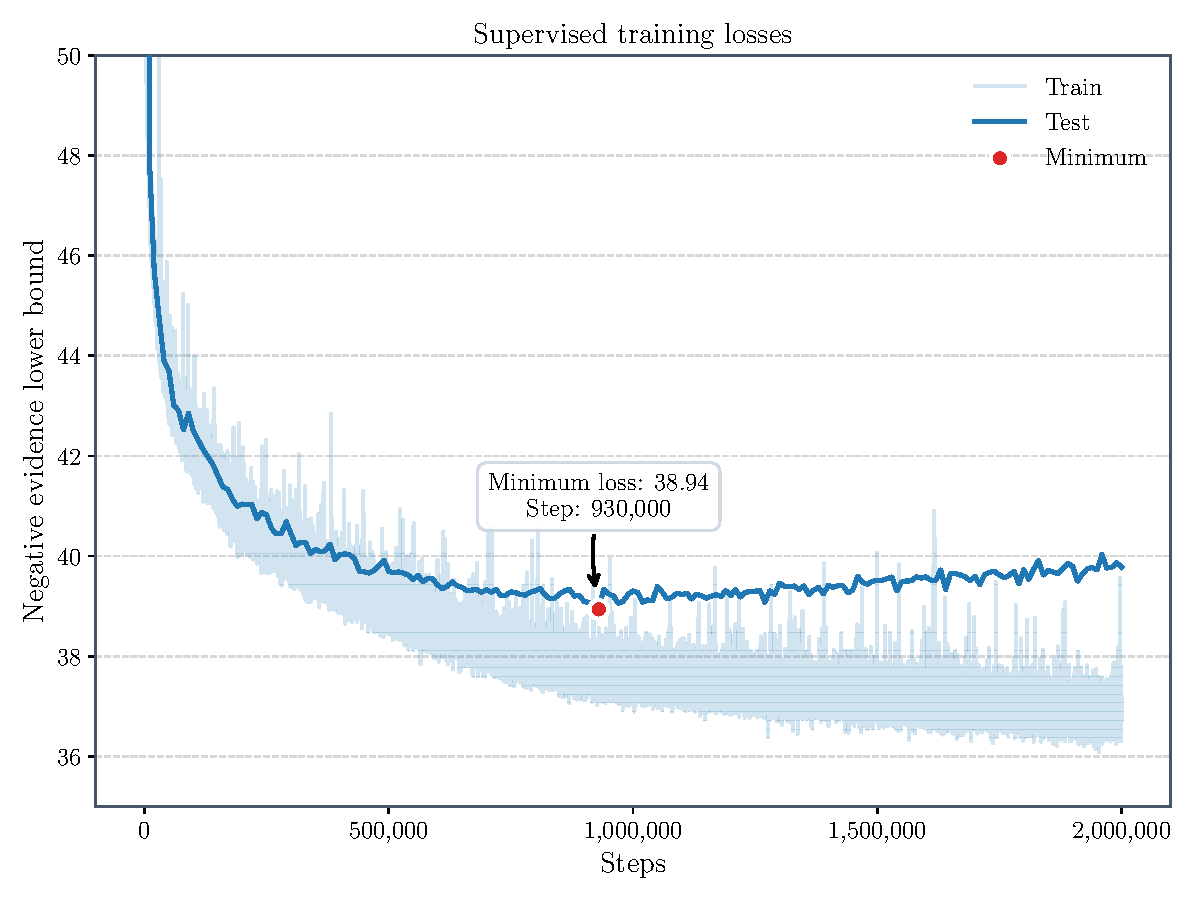
\includegraphics[width=0.75\textwidth]{./figures/supervised_training_progress/Training_loss.pdf}
        \caption{The negative evidence lower bound as a function of the training steps. After around 1,000,000, we observe overfitting.}
    \end{figure}
\end{frame}

\begin{frame}{Supervised results}
    \begin{figure}
        \centering
        
\includegraphics[width=0.49\linewidth]{./figures/supervised_training_progress/test/Legal_rate.pdf}
        \hfill
        
\includegraphics[width=0.49\linewidth]{./figures/supervised_training_progress/test/Uniqueness_rate.pdf}

        \caption{Evolution of the primary quality metrics with context from the test set during supervised pretraining. We omit the first data point, as it is identically zero for all metrics.}
    \end{figure}
\end{frame}

\begin{frame}{Supervised results}
    \begin{figure}
        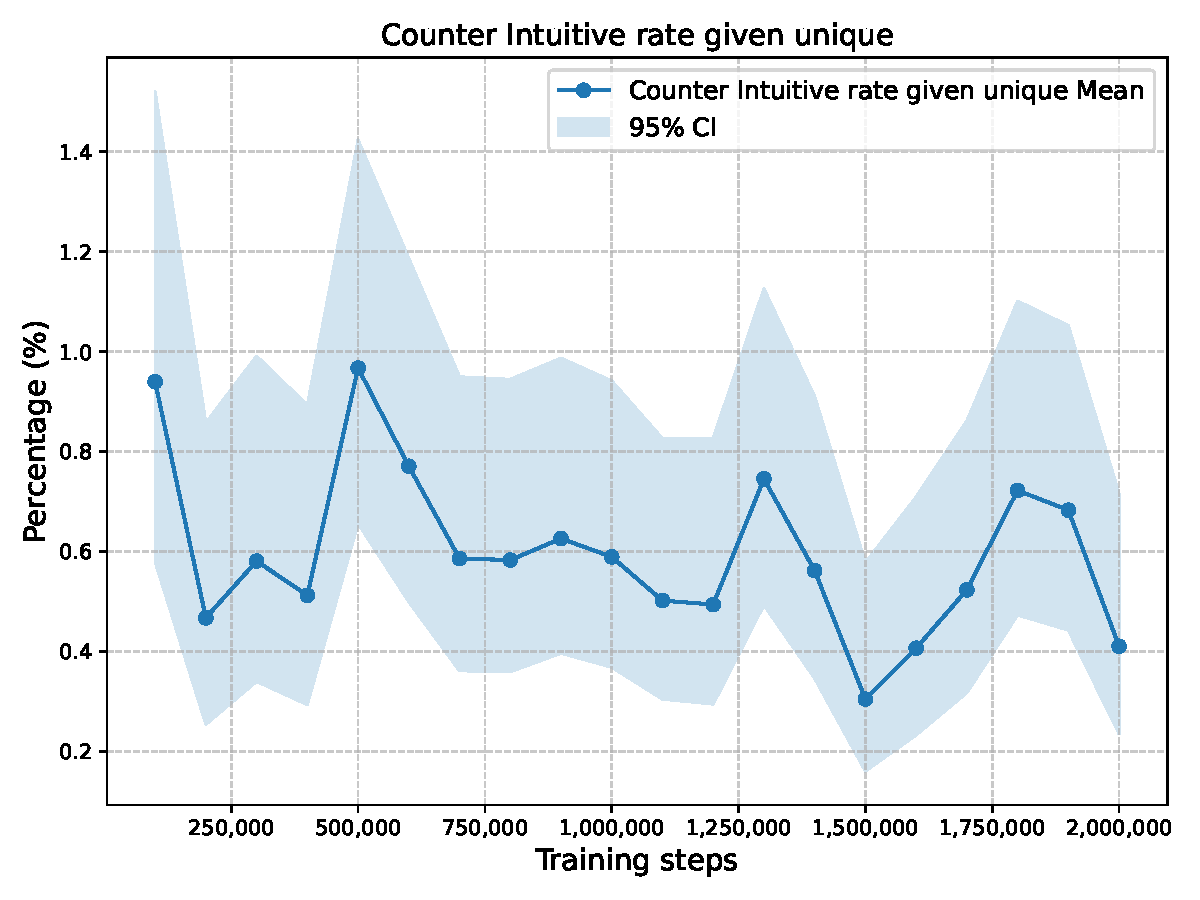
\includegraphics[width=0.49\linewidth]{./figures/supervised_training_progress/test/Counter_intuitive_rate_given_unique.pdf}
        \hfill
        
\includegraphics[width=0.49\linewidth]{./figures/supervised_training_progress/test/Puzzle_rate.pdf}

        \caption{Evolution of the primary quality metrics with context from the test set during supervised pretraining. We omit the first data point, as it is identically zero for all metrics.}
    \end{figure}
\end{frame}

\begin{frame}{Supervised results}
    \begin{table}
        \centering
        \caption{The final metrics after supervised training with different context distributions. The sampling is performed with a temperature 1.0 and 256 denoising steps. The errors are computed as the 95\% confidence intervals of the wanted proportion \cite{brown2001intervalestimationforabinomialproportion}.}
        \resizebox{\textwidth}{!}{
        \begin{tabular}{|c|c|c|c|c|c|}
            \hline
            Sampling & Legal & Unique & Counter-intuitive | unique & Puzzle & Theme\\
            \hline\hline
            block & 98.97 $\pm$ 0.044 & 27.08 $\pm$ 0.19 & 0.63 $\pm$ 0.018 & 0.17 $\pm$ 0.018 & 85.53 $\pm$ 0.18\\
            normal & 98.95 $\pm$ 0.045 & 28.75 $\pm$ 0.20 & 0.61 $\pm$ 0.018 & 0.18 $\pm$ 0.019 & 86.27 $\pm$ 0.19\\
            \hline\hline
            Lichess puzzles & \textbf{100.0} $\pm$ 0.0 & \textbf{83.58} $\pm$ 0.23 & \textbf{1.55} $\pm$ 0.070 & \textbf{1.29} $\pm$ 0.070 & \textbf{100.0} $\pm$ 0.0\\
            \hline
        \end{tabular}
        }
    \end{table}
\end{frame}

% \begin{frame}{Supervised results}
%     \begin{table}
%         \centering
%         \caption{The distance metrics after supervised training with different context distributions and sampling methods. The sampling is performed with a temperature 1.0 and 256 denoising steps. The self distances are computed with 40,000 samples and the Lichess distances with 100,000 samples. All generated positions are filtered so that we only compare positions that pass the uniqueness check.}
%         \resizebox{\textwidth}{!}{
%         \begin{tabular}{|c|c|c|c|c|}
%             \hline
%             Sampling & Board (Self) & Board (Lichess) & PV (Self) & PV (Lichess) \\
%             \hline\hline
%             block & 11.4987 & 11.1264 & 0.8655 & 0.8918\\
%             normal & 11.5497 & 11.1641 & 0.8723 & 0.8938\\
%             \hline\hline
%             Lichess puzzles & 11.8827 & - & 0.9496 & -\\
%             \hline
%         \end{tabular}
%         }
%     \end{table}
% \end{frame}


\begin{frame}{Reinforcement learning results}
    \begin{figure}
        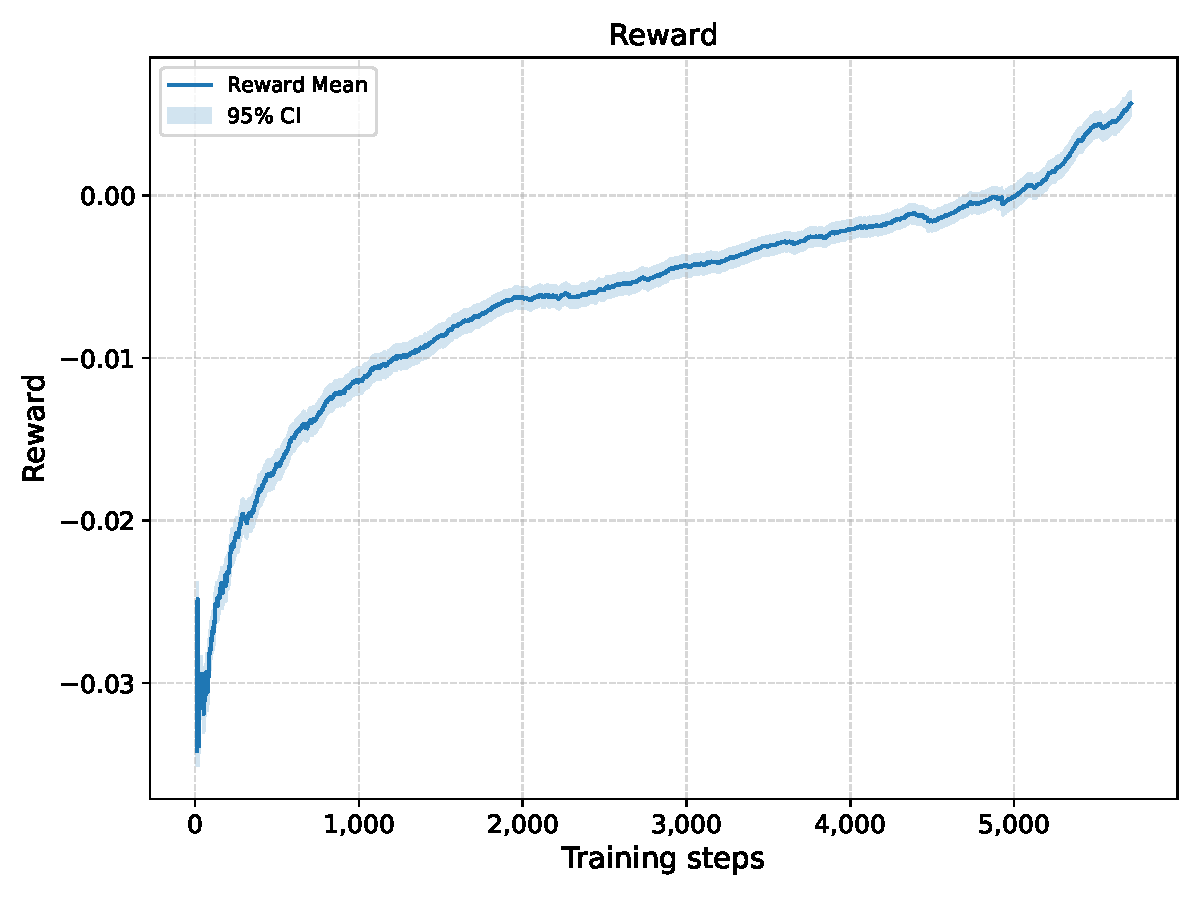
\includegraphics[width=0.24\textwidth]{./figures/rl_training_progress/good_run/Reward.pdf}
        \hfill
        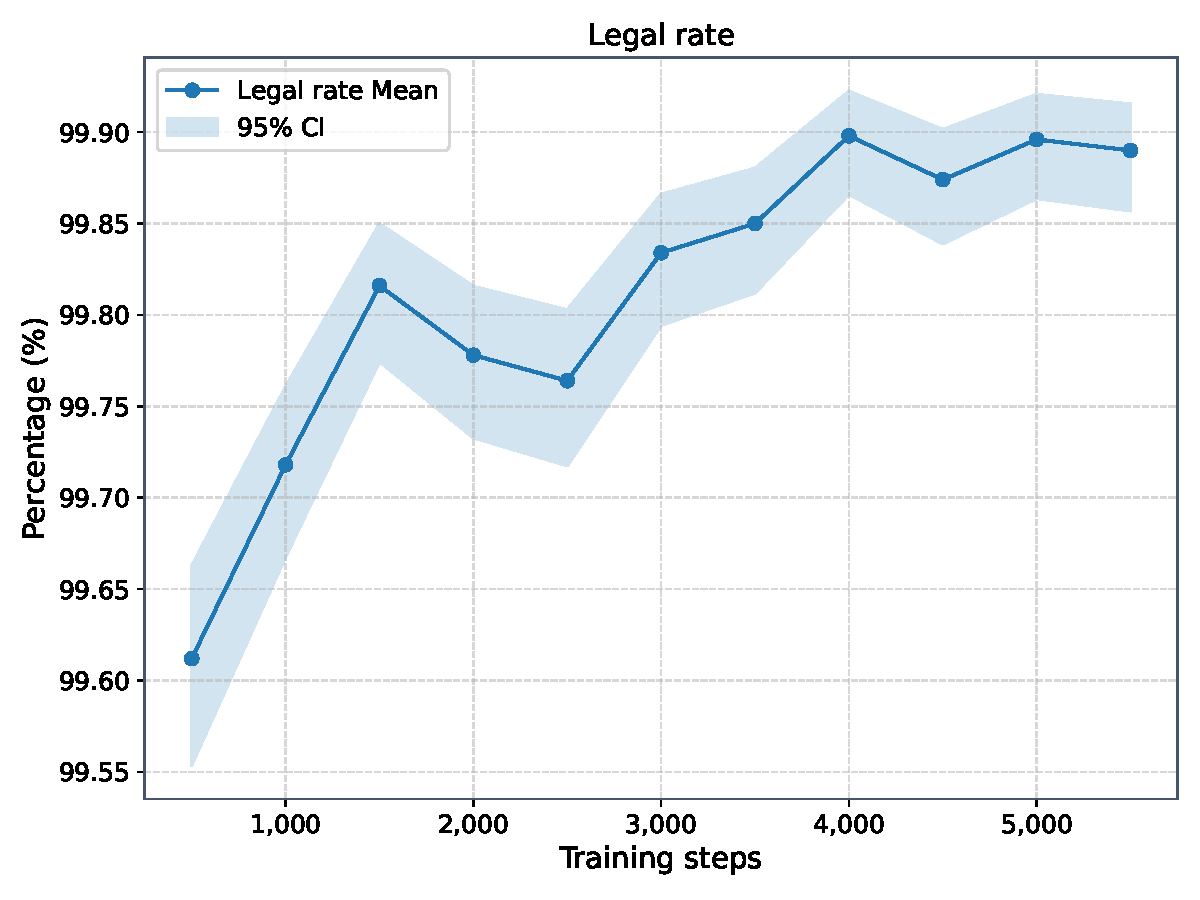
\includegraphics[width=0.24\textwidth]{./figures/rl_training_progress/good_run/Legal_rate.pdf}
        \hfill
        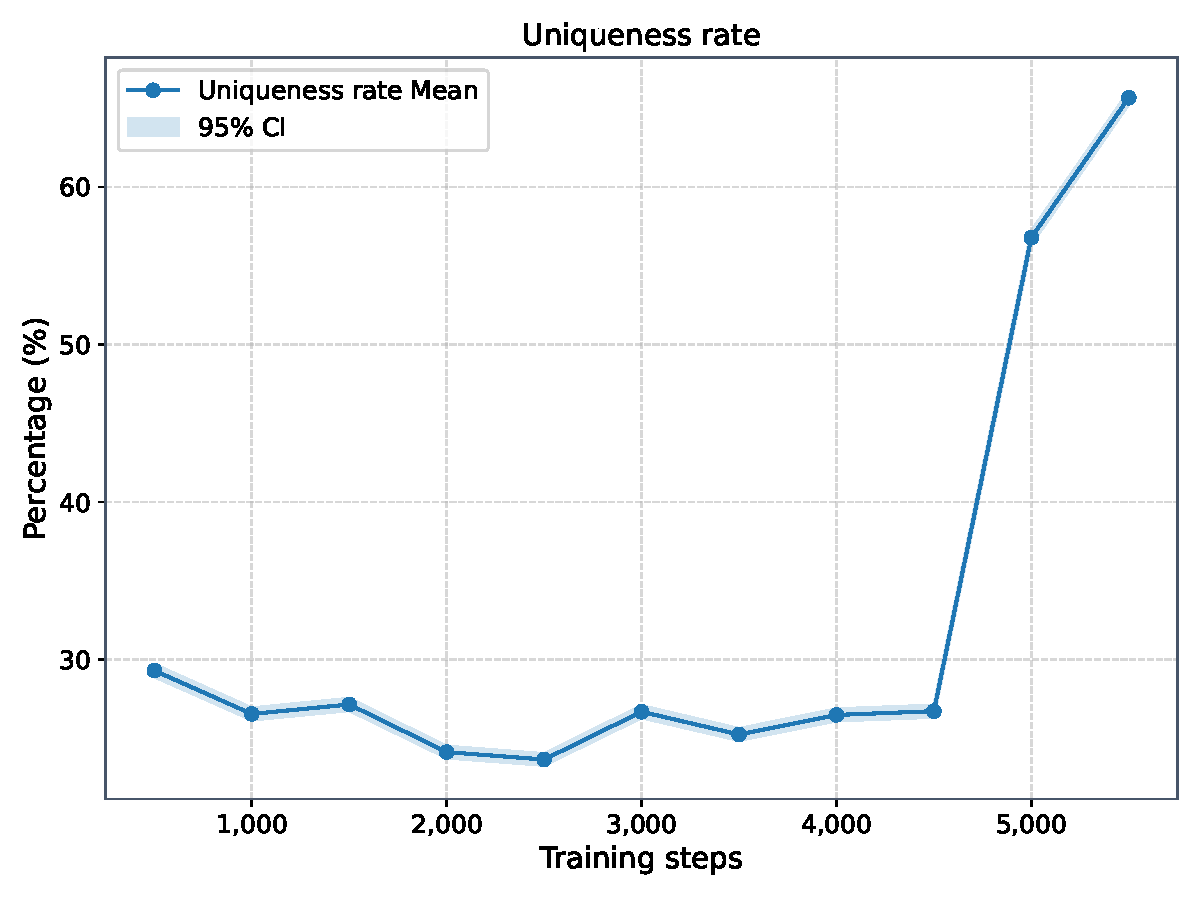
\includegraphics[width=0.24\textwidth]{./figures/rl_training_progress/good_run/Uniqueness_rate.pdf}
        \hfill
        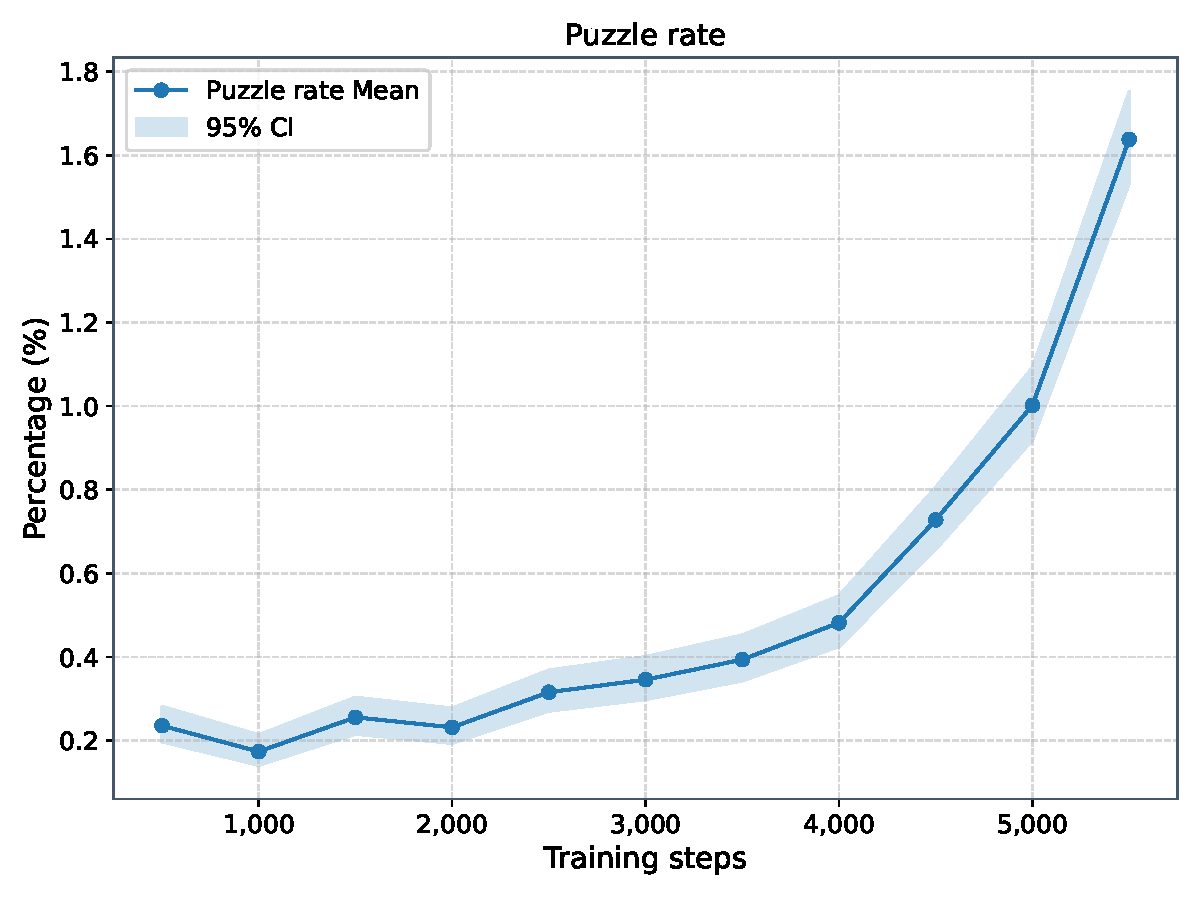
\includegraphics[width=0.24\textwidth]{./figures/rl_training_progress/good_run/Puzzle_rate.pdf}



        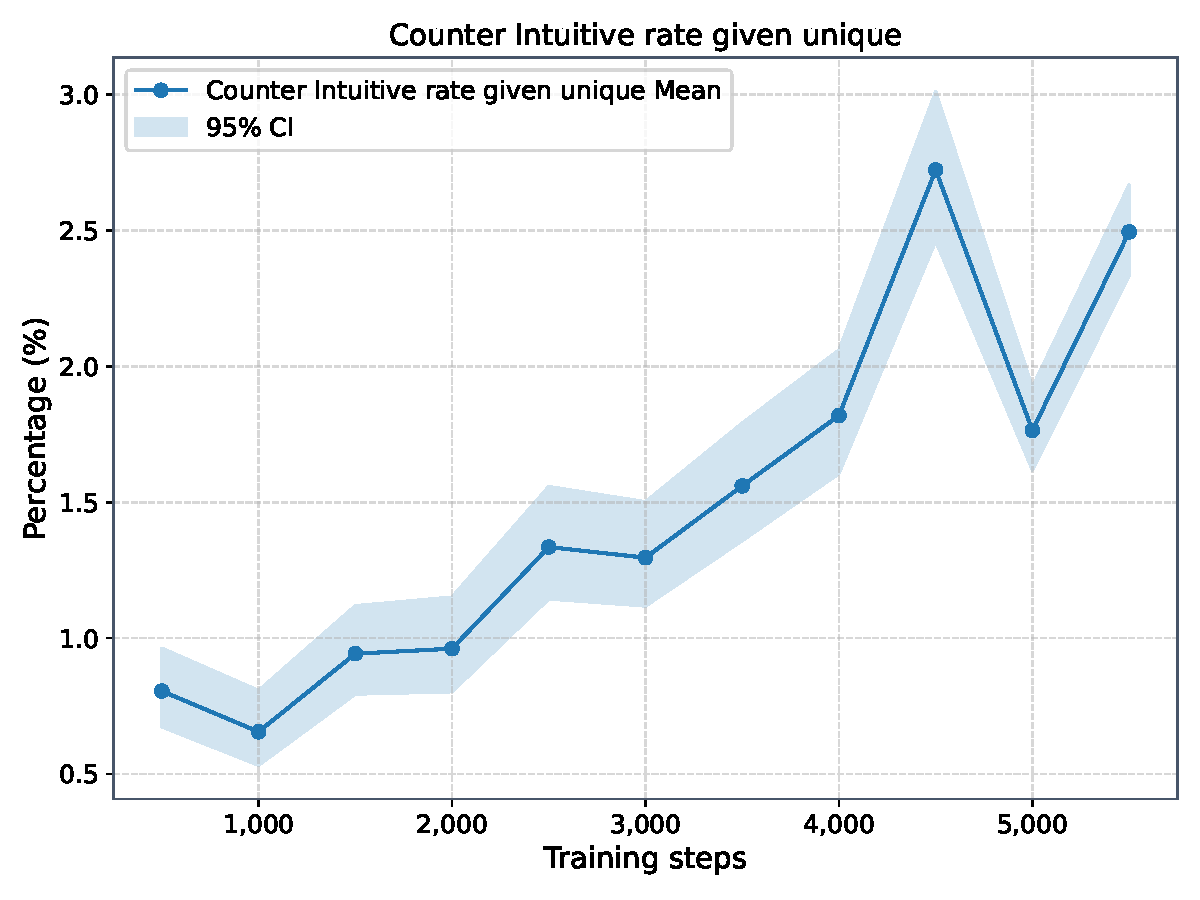
\includegraphics[width=0.24\textwidth]{./figures/rl_training_progress/good_run/Counter_Intuitive_rate_given_unique.pdf}
        \hfill
        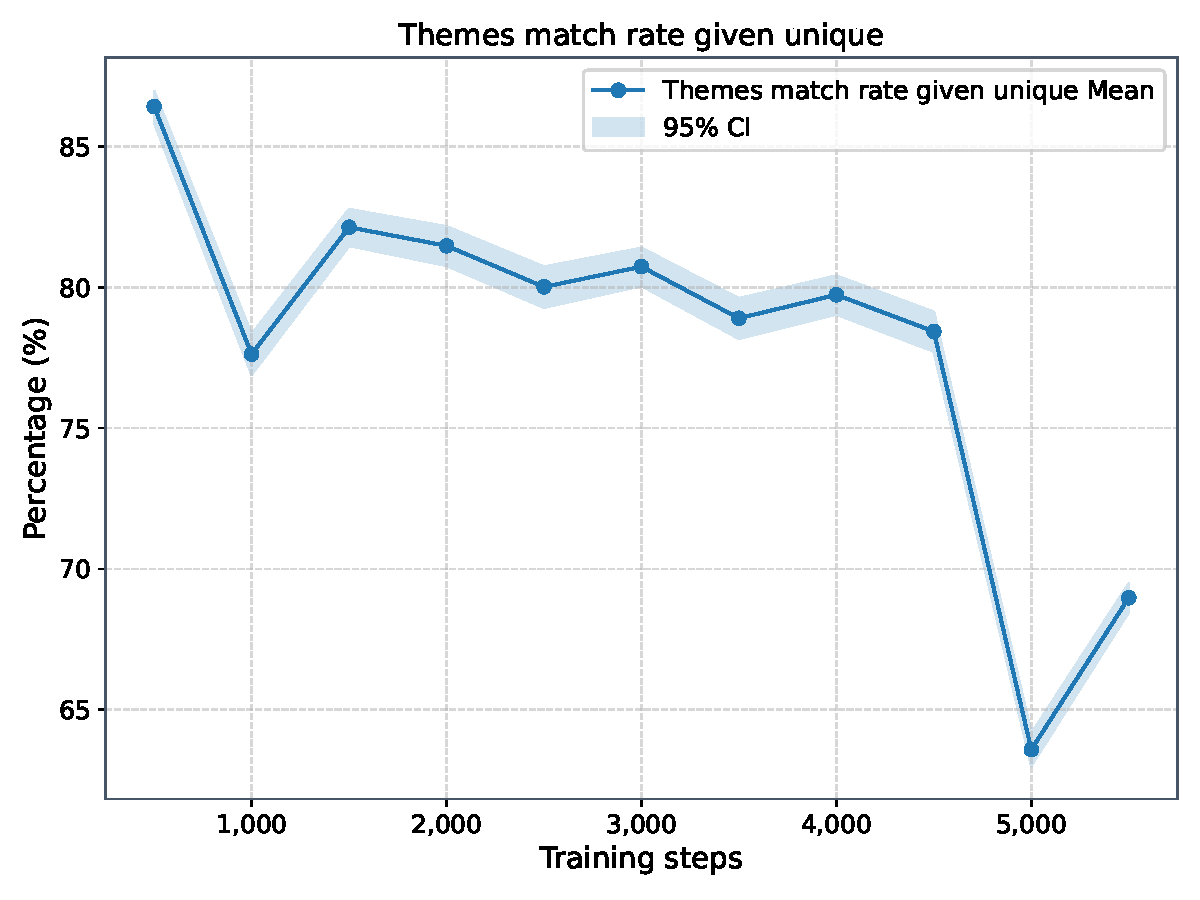
\includegraphics[width=0.24\textwidth]{./figures/rl_training_progress/good_run/Themes_match_rate_given_unique.pdf}
        \hfill
        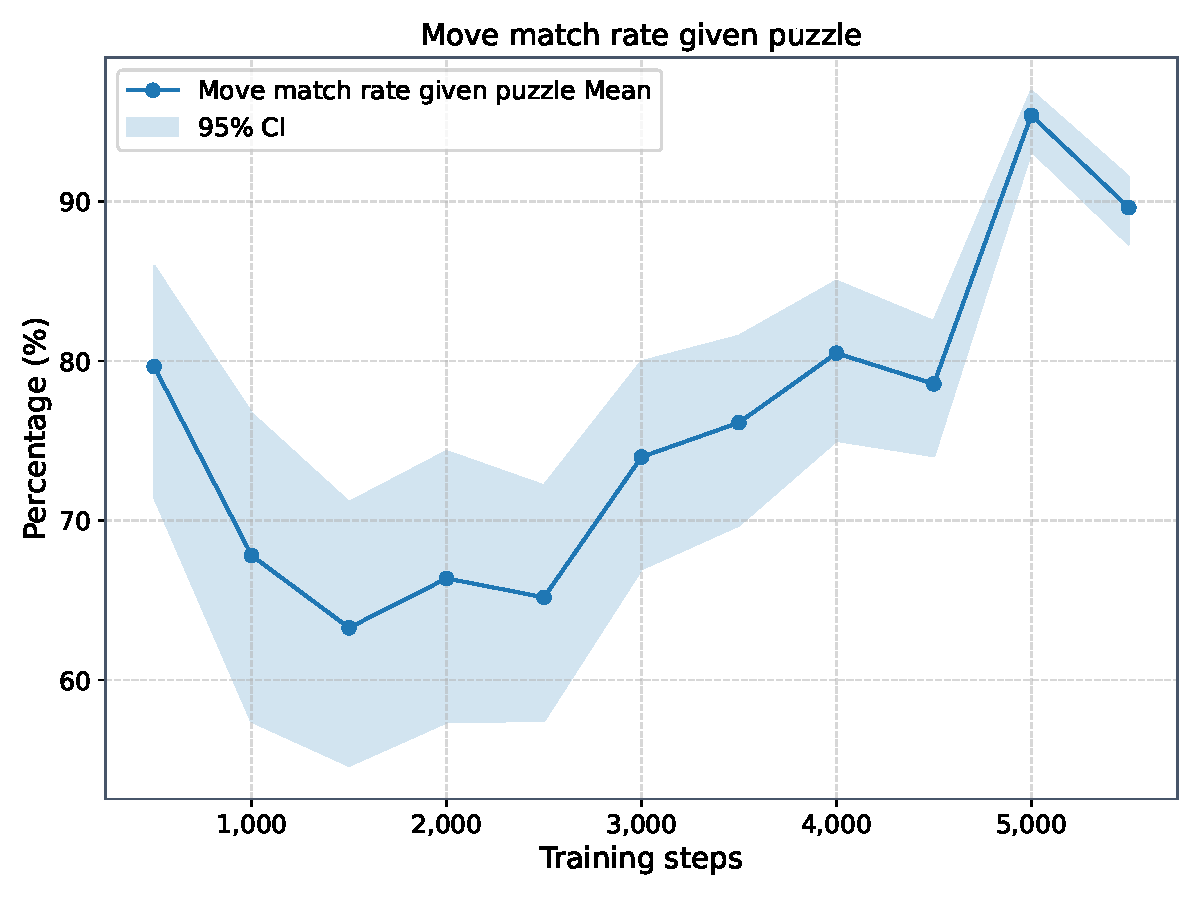
\includegraphics[width=0.24\textwidth]{./figures/rl_training_progress/good_run/Move_match_rate_given_puzzle.pdf}
        \hfill
        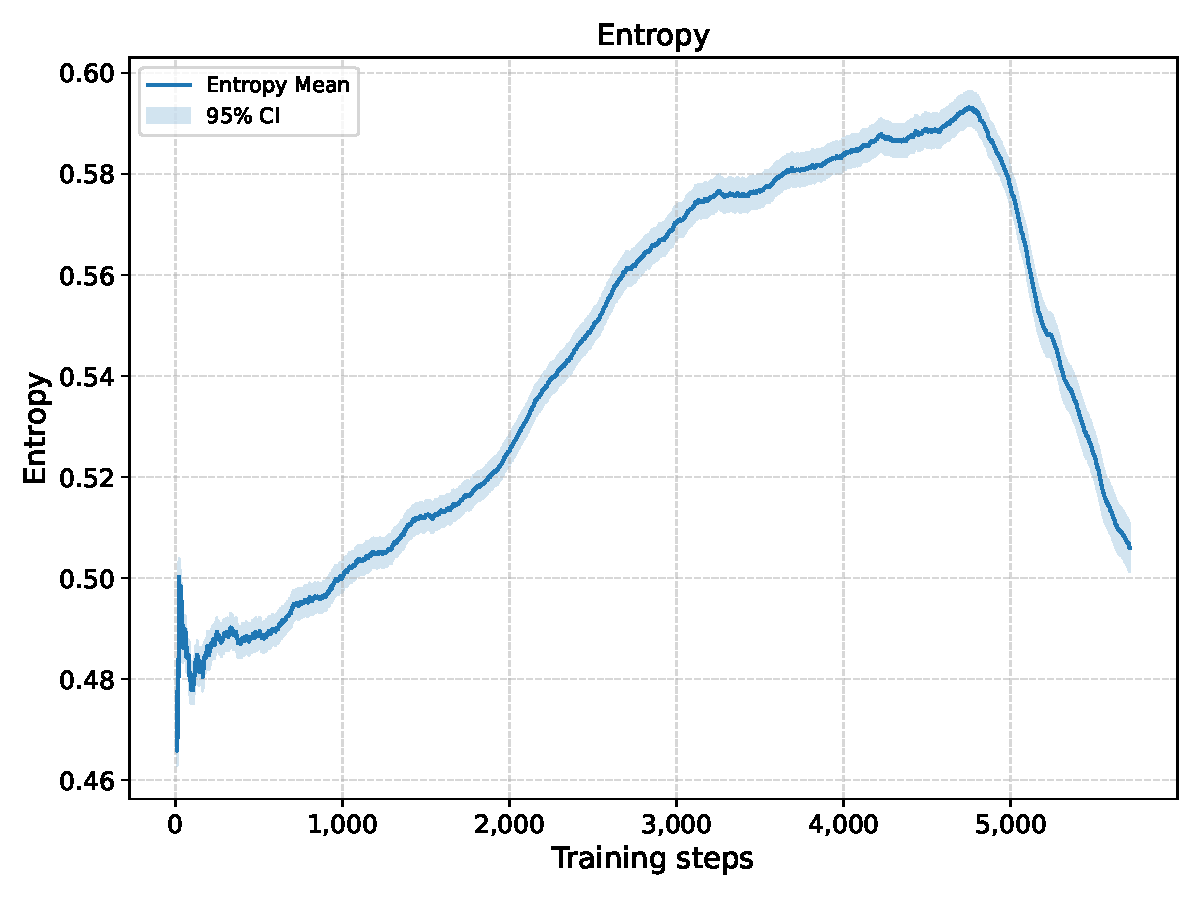
\includegraphics[width=0.24\textwidth]{./figures/rl_training_progress/good_run/Entropy.pdf}



        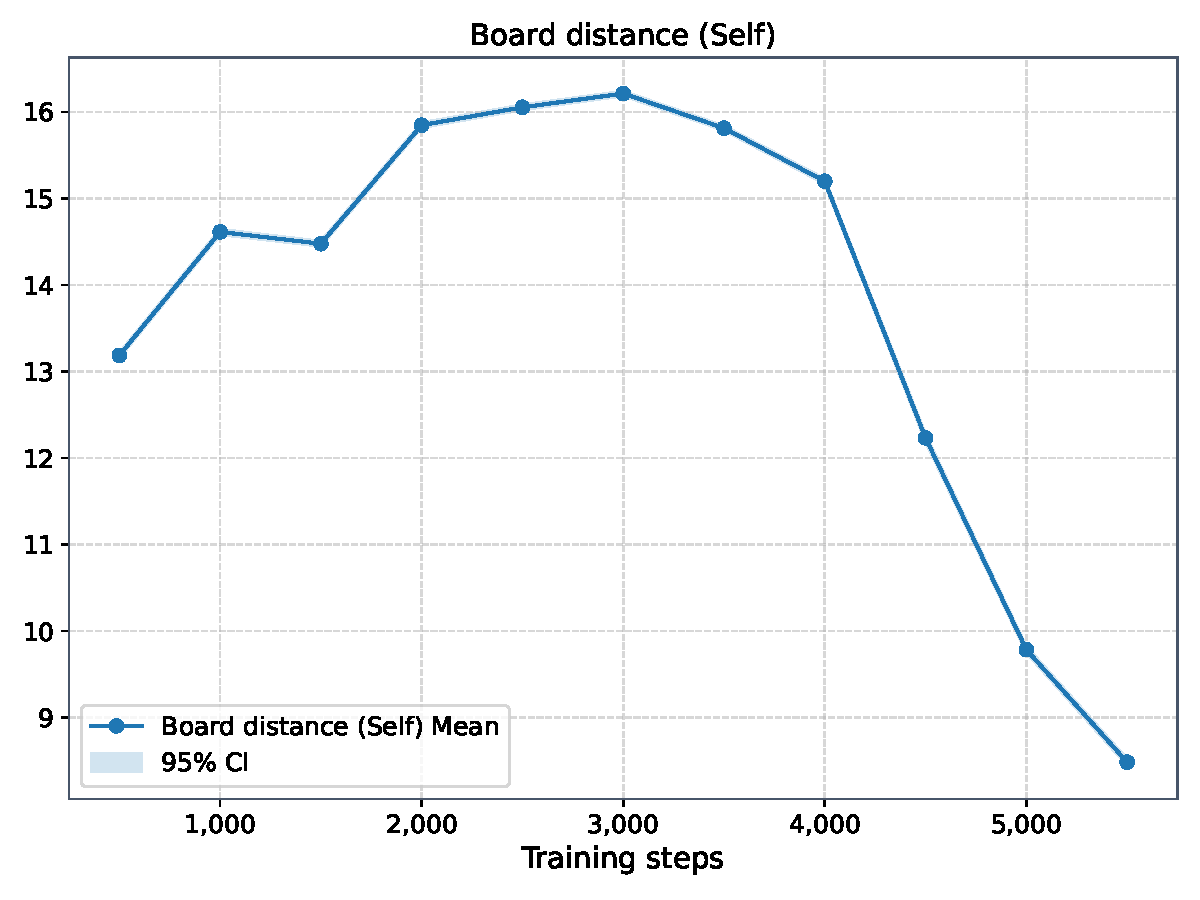
\includegraphics[width=0.24\textwidth]{./figures/rl_training_progress/good_run/self_distance_board.pdf}
        \hfill
        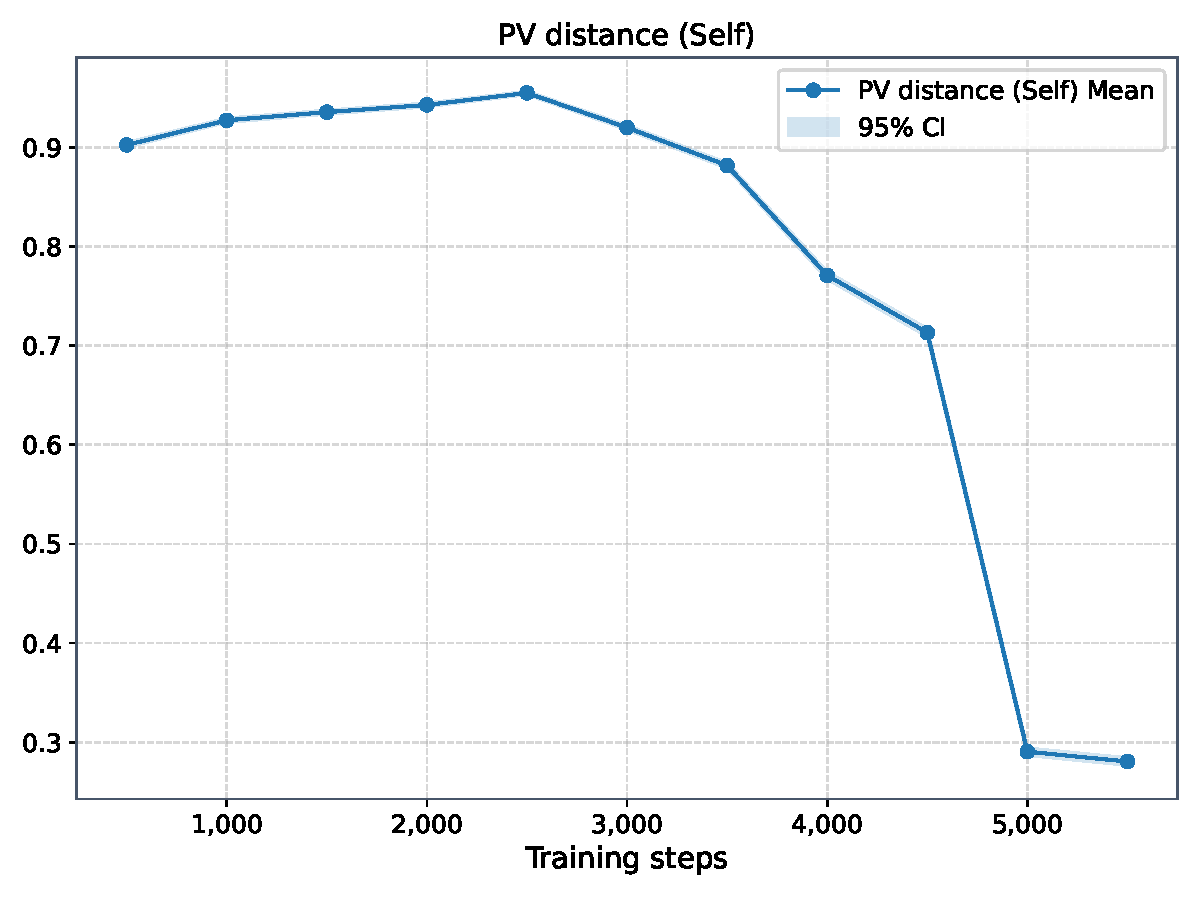
\includegraphics[width=0.24\textwidth]{./figures/rl_training_progress/good_run/self_distance_pv.pdf}
        \hfill
        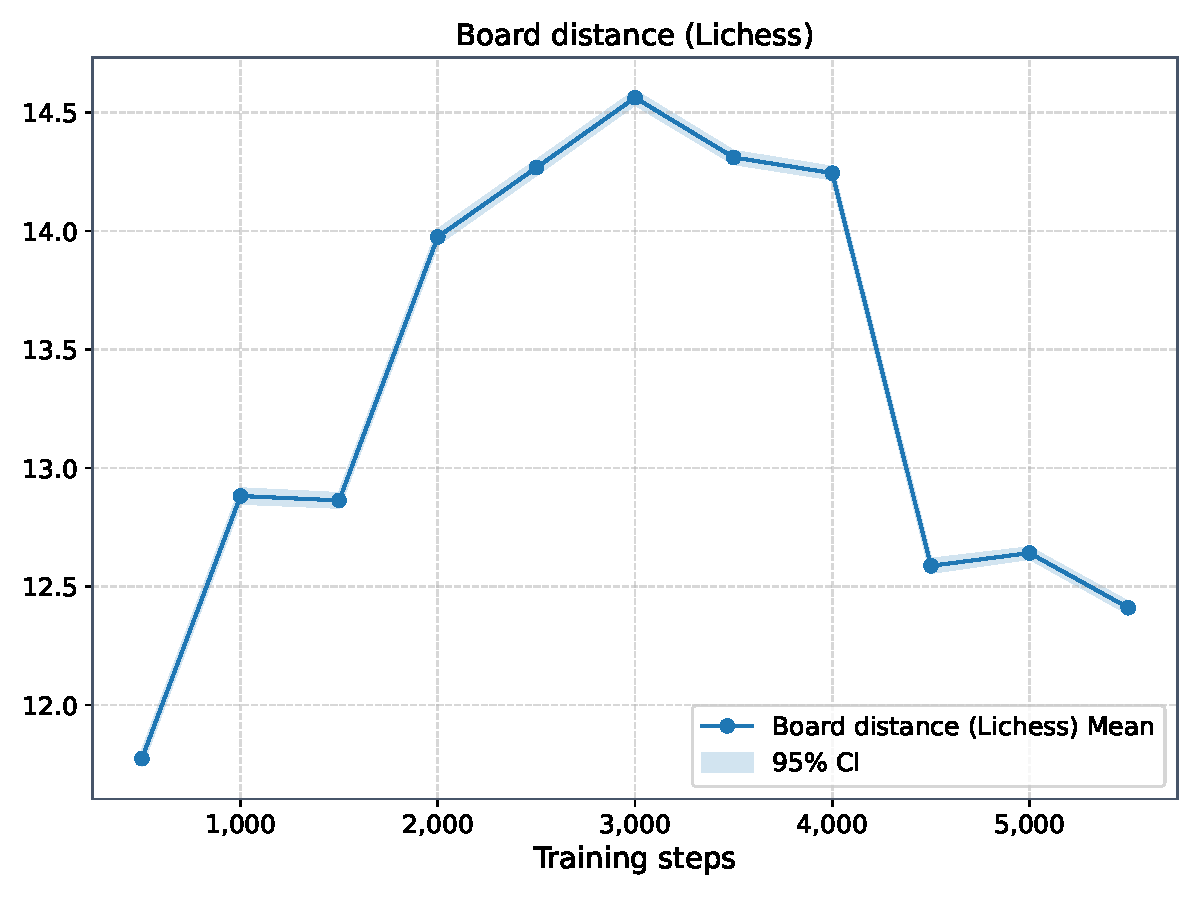
\includegraphics[width=0.24\textwidth]{./figures/rl_training_progress/good_run/lichess_distance_board.pdf}
        \hfill
        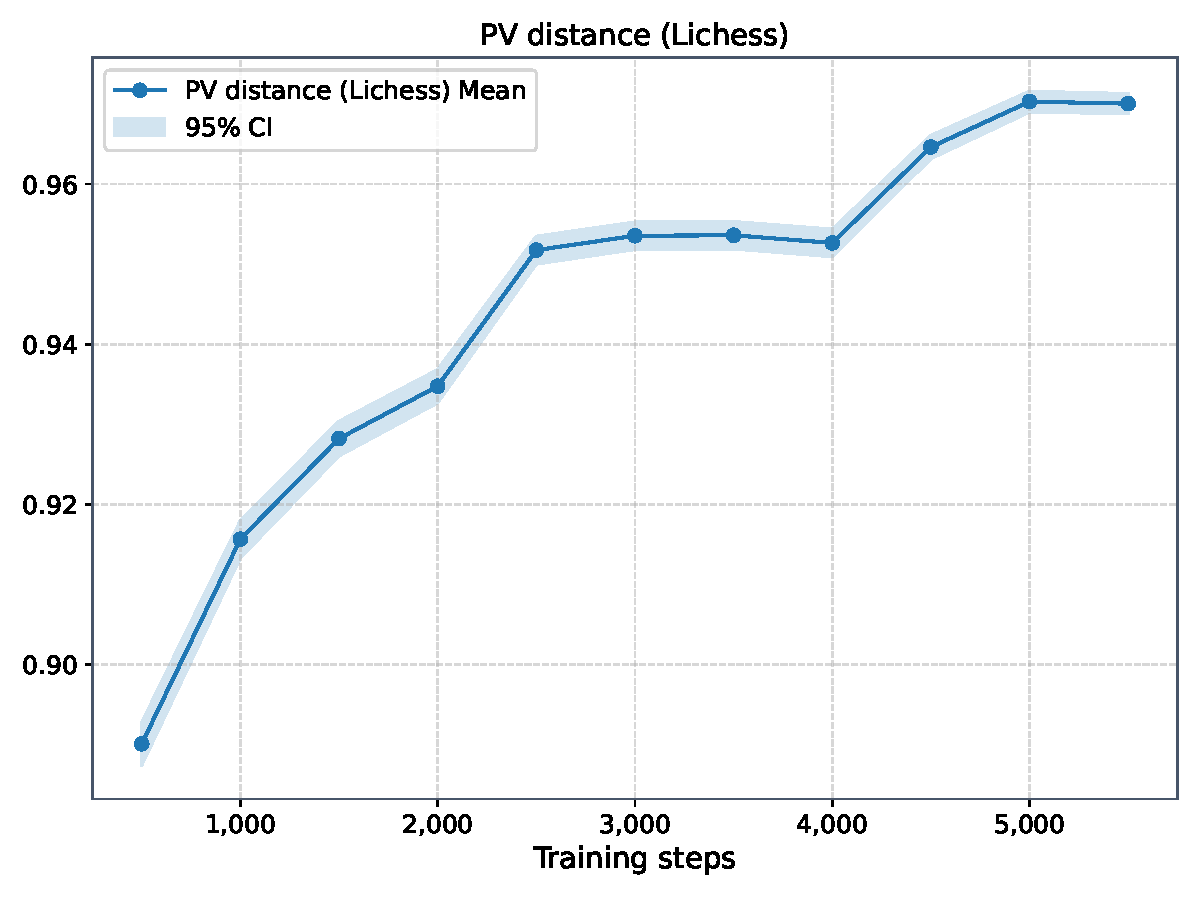
\includegraphics[width=0.24\textwidth]{./figures/rl_training_progress/good_run/lichess_distance_pv.pdf}
        
        \caption{The training progress during reinforcement learning. We observe model collapse after around 4,500 steps.}
    \end{figure}
\end{frame}

\begin{frame}{Reinforcement learning results}
    \begin{table}
        \centering
        \caption{The final metrics after RL training for 3,500 steps. The sampling is performed with a temperature 1.0 and 256 denoising steps. The errors are computed as the 95\% confidence intervals of the wanted proportion \cite{brown2001intervalestimationforabinomialproportion}.}
        \resizebox{\textwidth}{!}{
        \begin{tabular}{|c|c|c|c|c|c|}
            \hline
            Sampling & Legal & Unique & Counter-intuitive | unique & Puzzle & Theme\\
            \hline\hline
            normal & 99.87 $\pm$ 0.01 & 25.28 $\pm$ 0.09 & 1.45 $\pm$ 0.012 & 0.37 $\pm$ 0.012 & 78.72 $\pm$ 0.08\\
            \hline
        \end{tabular}
        }
    \end{table}
    % \begin{table}
    %     \centering
    %     \caption{The distance metrics after RL training for 3,500 steps. The self distances are computed with 40,000 samples and the Lichess distances with 100,000 samples.}
    %     \resizebox{\textwidth}{!}{
    %     \begin{tabular}{|c|c|c|c|c|c|}
    %         \hline
    %         Context & Sampling & Board (Self) & Board (Lichess) & PV (Self) & PV (Lichess) \\
    %         \hline\hline
    %         Test & normal & 15.0239 & 14.3468 & 0.8562 & 0.9533\\
    %         \hline
    %     \end{tabular}
    %     }
    % \end{table}
\end{frame}


\section{Conclusion}

\begin{frame}
\begin{center}
\Huge{\color{\thesiscolor} Conclusion}
\end{center}
\end{frame}

\begin{frame}{Conclusion}
    \begin{itemize}
        \item<1-> Masked diffusion models are an effective alternative to LLMs.
        \item<2-> Puzzle generation can be accurately conditioned on specific tactical themes.
        \item<3-> Performance of Masked diffusion models can be meaningfully improved through reinforcement learning, doubling the puzzle rate from 0.18\% to 0.37\%.
        \item<4-> Integrating the auxiliary task of predicting the best move enhances the generative capabilities.
        \item<5-> Future directions include generalization to other domains, exploring alternative RL algorithms (e.g., ESPO) and including chain-of-thought to puzzle generation.
    \end{itemize}
\end{frame}


\begin{frame}[allowframebreaks]{References}
    \bibliography{References.bib}
\end{frame}




\section{Example puzzles}

\begin{frame}{Example puzzles}
    \begin{columns}[t]
        \begin{column}{0.4\textwidth}
            \centering
            \chessboard[setfen=6k1/7p/pPp1P1pP/P4R2/6p1/r7/4r3/1K5R w - - 0 43, showmover=false, boardfontsize=12pt]
            \captionof{figure}{Example 1}
        \end{column}
        \hfill
        \begin{column}{0.4\textwidth}
            \centering
            \chessboard[setfen=r1b2k1r/2B1ppb1/p4np1/1p5p/1q3Pn1/PBN5/2P2QPP/3R1R1K w - - 1 22, showmover=false, boardfontsize=12pt]
            \captionof{figure}{Example 2}
        \end{column}
        \hfill
        \begin{column}{0.4\textwidth}
            \centering
            \chessboard[setfen=2r1k3/4qpp1/1p2P2p/pP1Q1p2/2Np4/P1r2R2/2P3P1/7K w - - 1 34, showmover=false, boardfontsize=12pt]
            \captionof{figure}{Example 3}
        \end{column}
    \end{columns}
\end{frame}

\begin{frame}{Example puzzles}
    \begin{columns}[t]
        \begin{column}{0.4\textwidth}
            \centering
            \chessboard[setfen=6k1/7p/pPp1P1pP/P4R2/6p1/r7/4r3/1K5R w - - 0 43, showmover=false, boardfontsize=12pt]
            \captionof{figure}{Example 1\footnotemark[1]}
        \end{column}
        \hfill
        \begin{column}{0.4\textwidth}
            \centering
            \chessboard[setfen=r1b2k1r/2B1ppb1/p4np1/1p5p/1q3Pn1/PBN5/2P2QPP/3R1R1K w - - 1 22, showmover=false, boardfontsize=12pt]
            \captionof{figure}{Example 2\footnotemark[2]}
        \end{column}
        \hfill
        \begin{column}{0.4\textwidth}
            \centering
            \chessboard[setfen=2r1k3/4qpp1/1p2P2p/pP1Q1p2/2Np4/P1r2R2/2P3P1/7K w - - 1 34, showmover=false, boardfontsize=12pt]
            \captionof{figure}{Example 3\footnotemark[3]}
        \end{column}
    \end{columns}

    \footnotetext[1]{Principal variation: f5b5 c6b5 b6b7}
    \footnotetext[2]{Principal variation: f2d2 b4d6 c7d6}
    \footnotetext[3]{Principal variation: e6f7 e8f8 c4e5 e7e5 d5e5}
\end{frame}



\end{document}

